\documentclass[11pt, titlepage]{article}
\usepackage[margin=1in]{geometry}
\usepackage[utf8]{inputenc}
\usepackage{titlepic}
\usepackage{graphicx}
\usepackage{hyperref}
\usepackage[toc,nonumberlist,acronym]{glossaries}

\linespread{1.5}

\makeatletter
\renewenvironment{thebibliography}[1]
     {\section*{\refname}%
      \@mkboth{\MakeUppercase\refname}{\MakeUppercase\refname}%
      \list{}%
           {\setlength{\labelwidth}{0pt}%
            \setlength{\labelsep}{0pt}%
            \setlength{\leftmargin}{\parindent}%
            \setlength{\itemindent}{-\parindent}%
            \@openbib@code
            \usecounter{enumiv}}%
      \sloppy
      \clubpenalty4000
      \@clubpenalty \clubpenalty
      \widowpenalty4000%
      \sfcode`\.\@m}
     {\def\@noitemerr
       {\@latex@warning{Empty `thebibliography' environment}}%
      \endlist}
\makeatother
\newcommand\frontmatter{
    \cleardoublepage
  \pagenumbering{roman}}

\newcommand\mainmatter{
    \cleardoublepage
  \pagenumbering{arabic}}

\title{Positive Train Control: Getting on the Right Track}
\titlepic{
    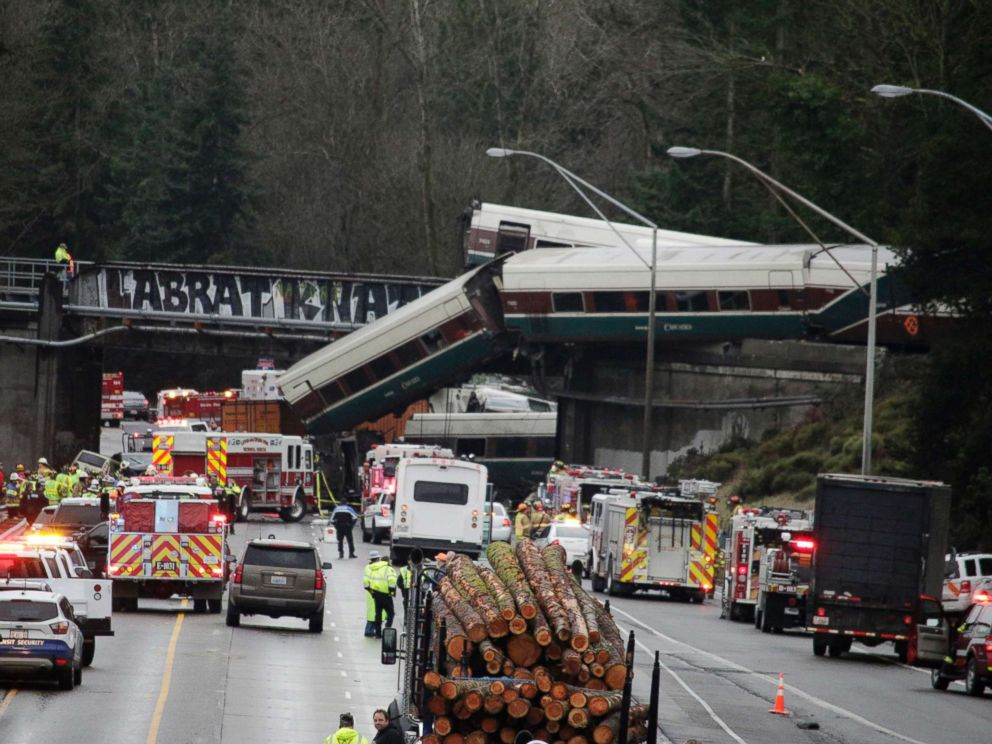
\includegraphics[width=5in]{TitleImage.png}\\
    (Citation)
}
\author{Michael Wu, Doruk Karınca, Austin Olson,\\Christian Clarion, John Song}
\date{March 19th, 2018}

\makeglossaries

\newacronym{fra}{FRA}{United States Federal Railroad Administration}
\newacronym{ptc}{PTC}{Positive Train Control}
\newacronym{gps}{GPS}{Global Positioning System}
\newacronym{ntsb}{NTSB}{National Transportation Security Board}
\newacronym{RSIA}{RSIA}{Railroad Safety Improvement Act}
\newacronym{USDOT}{USDOT}{United States Department of Transportation}
\newacronym{WMATA}{WMATA}{Washington Metropolitan Area Transit Authority}

\begin{document}

\maketitle

\frontmatter
\tableofcontents
\listoffigures
\listoftables

\mainmatter
\section{Executive Summary}

\pagebreak

\section{Introduction}

In preparing this report we initially divided our research between broad aspects of our topic. John and Michael decided to research the technological aspects of PTC, Doruk researched the economics behind PTC, Austin researched the laws regarding PTC, and Christian examined train crashes that could have prevented by PTC. After compiling sufficient information, we wrote short descriptions of our research individually. At this point, we had not yet received the course survival guide, and had no idea what the actual objective of our report was. In week eight of the quarter, we received the survival guide and drafted an outline for our report. We attempted to integrate our research into our technology and society sections of our outline. Then we brainstormed major ethical issues that were relevant to our topic and assigned writing sections for each group member.

We decided to include the train derailment cases that Christian researched in the background, John and Michael’s technical research in the technological issues section, and Austin and Doruk’s economic and legislative research in the ethical and societal issues section. For each ethical issue, we applied ethical frameworks to justify our reasoning about which course of action should be taken. Each member of our group discussed our ethical analysis with each other. We tried to separate our ethical analyses so that the person who researched an ethical issue the most provided analysis for that issue. Afterwards, we drew conclusions based on our ethical analysis and wrote recommendations for action.

Our editing process was done in person, and we met for a period of about six to seven hours as a group to finalize this report. During this time period, we wrote additional sections required for the final report such as the summary, introduction, and conclusion. After the bulk of our writing, we added images to help expand on our topic. We also compiled a glossary and table of contents. Our contribution matrix is shown below. X indicates primary contribution for a section.

\begin{table}[htbp]
    \begin{tabular}{r|c c c c c }
        & Doruk & John & Christian & Michael & Austin\\
        \hline
        Formatting & X & & & X & \\
        Executive Summary & X & & & & X \\
        Introduction & & & & X & \\
        Background & & & X & & X\\
        Technological Issues & & X & & X & \\
        Ethical and Societal Issues & X & X & X & X & X\\
        Recommendations & & & X & & X\\
        Conclusion & & X & X & & \\
    \end{tabular}
    \caption{Contribution Matrix}
\end{table}

\clearpage
\pagebreak

\section{Background}

\pagebreak

\section{Technological Issues}

\subsection{Technology of Historical Train Control Systems}

The earliest days of train control relied on simple signaling systems such as the manual block system. In this type of system, train operators relied on human signals such as telegraphs, paper, and voice to ensure that trains had appropriate space between each other (Thurston, 2012). Operators kept timetables that determined when trains should come and go, and control of the trains were manually enforced. The main concept in this type of system is the block, a section of railroad track that only one train can occupy at a time. If a train attempts to move into a block that is already occupied, operators signal for the train to stop until the block becomes vacant. Otherwise trains are free to move forward if the block ahead is not occupied. Blocks are long enough so that trains are kept a safe distance apart. Although this system ensures safety, it results in low efficiency and is prone to human error due to its manual nature.

Another type of manual train control system is the track warrant control system, where dispatchers give a train exclusive access to a section of rail through radio (Thurston, 2012). In this system, trains do not enter sections of rail unless told to do so. This ensures a higher standard of safety than the manual block system, as trains will not be able to access a rail unless explicitly given permission. But like the manual block system, the track warrant control system is not very efficient and cannot handle high throughput because it relies on human signals. This type of system is typically used on railroads that do not see a lot of traffic.

The modern equivalent of the manual block system is the automatic block system. Like the manual block system, this concept sections the rail into blocks that only one train can occupy at a time. But it uses electrical circuits to automatically turn on red or yellow wayside signals that indicate to oncoming trains to stop or slow down, rather than manually keeping track of where a trains are. These circuits are located on the tracks themselves, and are activated when a train makes contact with them. When a train passes a red or yellow signal, the automatic block system can cause the train to decrease its speed appropriately. This allows for greater capacity of trains on a given track, which leads to increased efficiency. Automatic block signalling is the most common system employed today for freight lines (Thurston, 2012). A more advanced version of this is cab signalling, where the signals for blocks on a line are constantly relayed to the interior of each train. With cab signalling, drivers of the trains can more easily see the status of blocks on the rail network. Instead of having to check the wayside signals next to the track when they pass by, they can check the block signals at any time.

Modern train control systems can also include emergency stops, such as a trip stop. If a train passes over a red signal while entering a block, the trip stop will trigger the emergency brakes. This can be implemented mechanically, where a trip arm comes in contact with the train to activate the brakes. It can also be implemented magnetically, where an electromagnet activates the brakes (Thurston, 2012). Including trip stops means that trains need more space between them than the space required in a signalling only system, because this is necessary to avoid an accidental trigger of the stop. These trip stops are limited in enforcing control, as they can only work at locations where a wayside signal is present. In between the locations where the signals are, the stops cannot trigger the emergency brakes and cannot prevent accidents.

\subsection{Technology Behind PTC}

\begin{figure}[h]
    \begin{center}
        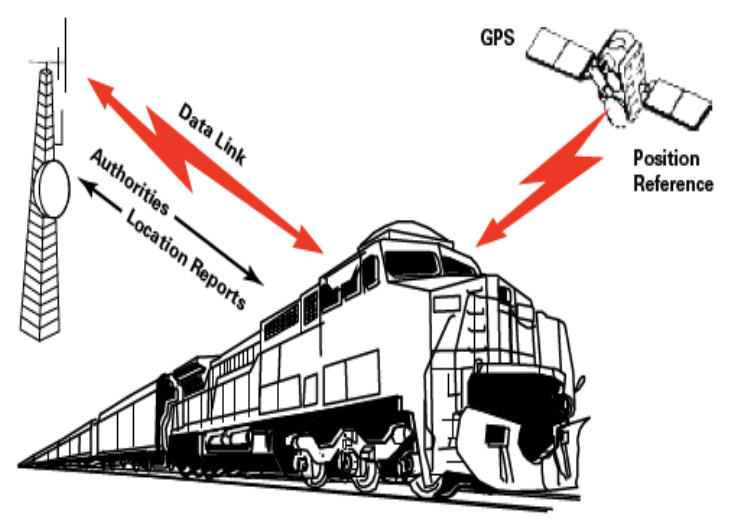
\includegraphics[width=4in]{PTCDiagram.png}
        \caption{Implementation of PTC (Badugu, 2013).}
    \end{center}
\end{figure}

PTC represents the newest technology in train control, and functions much differently from previous signal-based control systems. This type of system relies on GPS and wireless communications to a train’s computer to determine how to adjust its speed or stop accordingly. Trains check in with a centralized control tower that tells them what to do. The central authority can tell a train to reduce its speed if it comes too close to another train, exceeds the maximum speed limit, or approaches hazardous sections of rail. This type of system does not rely on circuits on the tracks to detect the position of the trains, leading to more robust handling and control. Thus the PTC system will enable train operators to have real time information about train location in ``dark territory'', where track circuits are not installed. Additionally, instead of relying on fixed blocks PTC can ``establish moving blocks around trains, providing sufficient separation between moving trains to ensure maximum track utilization'' (Badugu, 2013). In many ways, PTC behaves similarly to modern air traffic control systems. Currently PTC acts as an additional safety measure on top of existing train control technologies, but in the future it may become the primary means of train control.

Components of a typical PTC system will include technology inside each train, technology inside a control center, and a communication link between each train and the control center. Inside each train, there must be some device to obtain its position. This can be a GPS receiver or a receiver that obtains signals from wireless location devices alongside the train tracks. Software on the train uses the position information to calculate if braking is necessary based on the its current speed and its location on the tracks. Onboard computers store speed limit profiles for the train tracks and information about the train’s stopping capabilities to make these calculations (Badugu, 2013). Because this feature can be implemented onboard, constant communication with the central authority is not necessary to enforce speed limits. The central authority is only necessary to update stored speed limit profiles, which may be done intermittently.

Inside the control center, there must be technology to monitor the locations of each train in the rail system. Communication between the control center and trains is achieved through wireless signals, allowing a control center to cover a large number of moving trains in a given system. The central authority issues movement authorizations for each train based on their relative locations. If a train begins to move outside its authorized movement zone, the control center will issue a warning to notify the train operator, who should correct the train’s movement. If the engineer does not do so, the control center will give a signal for the train to automatically brake. The control center can also monitor track circuits, wayside signals, and switches on the tracks to prevent crashes. By doing so, the control center can detection more hazards on the tracks and stop trains in more cases. However, this is an optional part of PTC and is not necessarily present in all PTC systems. PTC cannot detect some hazards such as obstructions, flooding, or broken rails without knowledge of track circuits.

\subsection{Technical Challenges of PTC}

\subsubsection{Negative Effects on Performance}

Another concern about implementing PTC is whether or not it will negatively affect railway performance. Although PTC might provide greater safety, it could also be too restrictive and unnecessarily slow down trains. In the past, ``the freight railroad industry has been reluctant to fit speed control devices due to the often heavy-handed nature of such devices having an adverse effect on otherwise safe train operation'' (Badugu, 2013). Historically, trains have relied only on signals and human judgment to ensure safety. If trains have been operating safely this way for decades, why limit the power of train operators who are experienced in properly controlling their vehicles? Implementing PTC may mean that train operators must slow down when they know that it is safe to proceed, reducing the efficiency of a railroad line. The FRA has recognized this challenge, and even admitted in 2009 that ``PTC was in fact likely to decrease the capacity of freight railroads on many main lines'' (Badugu, 2013). Thus engineers must work to design PTC systems that allow for the same, or even better, levels of efficiency as signalling systems.

\pagebreak

\section{Ethical and Social Issues}

\pagebreak

\section{Recommendations}

\pagebreak

\section{Conclusion}

\pagebreak

\glsaddall
% \printglossaries % uncomment to regenerate glossary
\printglossary[title=Definitions,type=\acronymtype]

\phantomsection
\addcontentsline{toc}{section}{References}
\begin{thebibliography}
    \raggedright
    \bibitem{badugu} Badugu, S., and Movva, A., April, 2013, Positive Train Control; International Journal of Emerging Technology and Advanced Engineering, v. 3, issue no. 4.
    
    \bibitem{thurston} Thurston, D.F., May, 2012, A Proactive Approach To Train Control; Temple University, ProQuest Dissertations Publishing.
\end{thebibliography}

\end{document}
